\documentclass[12pt]{article}

%------------- PREAMBLE -------------
\usepackage[margin=1in]{geometry}
\usepackage{amsmath,amssymb,mathtools}
\usepackage{enumitem}
\usepackage{bm}
\usepackage{hyperref}
\usepackage{fancyhdr}
\usepackage{draftwatermark}
\usepackage{xcolor}
\usepackage{titlesec}
\usepackage{tikz}
\usetikzlibrary{arrows.meta,calc,positioning}

%------------- TITLE AND METADATA -------------
\newcommand{\CourseCode}{MH1301}
\newcommand{\CourseName}{Discrete Mathematics}
\newcommand{\DocType}{Tutorial 9}

\title{
\CourseCode\ \CourseName \\[0.3em]
\large \DocType
}
\author{
  Academic Year 2025/2026, Semester 2 \\[0.25em]
  \textit{Quantitative Research Society @NTU}
}
\date{\today}

%------------- HEADER & FOOTER (for page 2 onward) -------------
\fancypagestyle{main}{
  \fancyhf{}
  \fancyhead[L]{\CourseCode\ \CourseName}
  \fancyhead[R]{\href{https://qrsntu.org}{QRS@NTU}}
  \fancyfoot[C]{\thepage}
  \renewcommand{\headrulewidth}{0.4pt}
  \renewcommand{\footrulewidth}{0pt}
}

%------------- SIMPLE FOOTER (page 1 only) -------------
\fancypagestyle{plainfirst}{
  \fancyhf{}
  \renewcommand{\headrulewidth}{0pt}
  \renewcommand{\footrulewidth}{0pt}
  \fancyfoot[C]{\scriptsize\textcolor{gray}{\textit{For academic reference only. This document is provided for educational purposes and does not constitute an official question paper, answer key, or any formally authorised academic material. Its content is not guaranteed to be complete or accurate.}}}
}

%------------- WATERMARK -------------
\SetWatermarkText{Unofficial --- QRS@NTU --- qrsntu.org}
\SetWatermarkScale{1}
\SetWatermarkLightness{0.985}

%------------- SHORTCUTS -------------
\newcommand{\N}{\mathbb{N}}
\newcommand{\Z}{\mathbb{Z}}
\newcommand{\R}{\mathbb{R}}
\newcommand{\comp}[1]{\overline{#1}}
\newcommand{\V}{V}
\newcommand{\E}{E}
\newcommand{\degG}{\deg}
\newcommand{\diam}{\operatorname{diam}}
\newcommand{\blankedge}{\text{--}}
\newcommand{\edge}[2]{#1#2}

\DeclareMathOperator{\dist}{dist}

\tikzset{
  vtx/.style={circle, draw, minimum size=20pt, inner sep=1pt},
  dotv/.style={circle, fill, inner sep=1.4pt},
  every picture/.style={line cap=round, line join=round}
}

\setcounter{secnumdepth}{-1}
\setcounter{tocdepth}{3}
\setlist[enumerate]{itemsep=0.3em, topsep=0.3em}
\setlist[itemize]{itemsep=0.2em, topsep=0.2em}
\setlength{\headheight}{14.5pt}

\begin{document}

%------------- COVER PAGE -------------
\maketitle
\thispagestyle{plainfirst}
\pagestyle{main}

%====================================================
% OVERVIEW
%====================================================
\begin{center}
  \rule{0.82\textwidth}{0.4pt}\\[4pt]
  \textbf{Overview}\\[2pt]
  \rule{0.82\textwidth}{0.4pt}
\end{center}

\noindent
This tutorial develops graph-theoretic tools for bipartite graphs, planar graphs, and graph colourings, with emphasis on:
\begin{itemize}[leftmargin=*]
  \item Hamilton paths and Euler-path feasibility via degree conditions;
  \item bipartite graph recognition using explicit bipartitions and odd-cycle obstructions;
  \item degree sequences of complete bipartite graphs;
  \item planarity of graphs obtained from $K_{3,3}$ and $K_5$ by deleting one edge;
  \item planar examples with chromatic number $4$ and vertex-deletion behaviour of chromatic number;
  \item planar drawings of utility graphs and a given six-vertex graph;
  \item extremal examples for chromatic number after deleting an arbitrary vertex.
\end{itemize}

\noindent
\textbf{Question map.}
\begin{itemize}[leftmargin=*]
  \item Question 1: Hamilton paths, Euler paths, and degree-sequence feasibility.
  \item Questions 2--4: bipartite graphs and degree sequences.
  \item Questions 5, 7, and 8: planar drawings and planarity certificates.
  \item Questions 6 and 9: chromatic number, planar examples, and vertex deletion.
\end{itemize}

\newpage
\tableofcontents
\newpage

%====================================================
% QUESTION 1
%====================================================
\section{Question 1 (Hamilton paths, Euler paths, and degree sequences)}

\subsection{Problem}
\begin{enumerate}[label=(\alph*)]
  \item How many edges are on a Hamilton path?
  \item Is there a connected graph with an Euler path that has the degree sequence
  \[
  4,4,2,1,1?
  \]
\end{enumerate}

\subsection{Solution}

\subsubsection{Method 1: Direct vertex-count and degree obstruction}
\begin{enumerate}[label=(\alph*)]
  \item Suppose the graph has $n$ vertices. A Hamilton path visits every vertex exactly once. Therefore its vertices can be written in the form
  \[
  v_1,v_2,\dots,v_n,
  \]
  where $v_i\neq v_j$ for $i\neq j$, and its edges are exactly
  \[
  v_1v_2,
  v_2v_3,
  \dots,
  v_{n-1}v_n.
  \]
  Hence the number of edges on the Hamilton path is
  \[
  n-1.
  \]
  Thus
  \[
  \boxed{\text{a Hamilton path on }n\text{ vertices has }n-1\text{ edges}.}
  \]

  \item Suppose such a graph $G$ exists. The degree sequence has five entries, so $|V(G)|=5$. Let $u$ and $v$ be the two vertices of degree $4$.

  Since $G$ is simple and has $5$ vertices, a vertex of degree $4$ is adjacent to every other vertex. Hence every vertex other than $u$ is adjacent to $u$, and every vertex other than $v$ is adjacent to $v$.

  In particular, any vertex $w\notin\{u,v\}$ is adjacent to both $u$ and $v$. Therefore
  \[
  \deg(w)\ge 2.
  \]
  But the proposed degree sequence contains two vertices of degree $1$, contradiction.

  Therefore no simple graph has this degree sequence. Consequently, there cannot be a connected graph with an Euler path and this degree sequence.
  \[
  \boxed{\text{No such connected graph exists.}}
  \]
\end{enumerate}

\subsubsection{Method 2: Havel--Hakimi graphicality test and Euler-path criterion}
\textbf{Theorem/criterion used.} The Havel--Hakimi reduction says that a nonincreasing sequence
\[
 d_1,d_2,\dots,d_n
\]
of nonnegative integers is graphical if and only if the sequence obtained by deleting $d_1$ and subtracting $1$ from the next $d_1$ entries is graphical, after reordering. A negative entry proves that the sequence is not graphical.

\begin{enumerate}[label=(\alph*)]
  \item A Hamilton path has one edge between each consecutive pair in an ordering of all $n$ vertices:
  \[
  v_1v_2,\ v_2v_3,\ \dots,\ v_{n-1}v_n.
  \]
  Hence there are $n-1$ such consecutive pairs. Therefore
  \[
  \boxed{\text{a Hamilton path has }n-1\text{ edges}.}
  \]

  \item Apply Havel--Hakimi to
  \[
  4,4,2,1,1.
  \]
  Delete the first $4$ and subtract $1$ from the next four entries:
  \[
  (4,2,1,1)\mapsto (3,1,0,0).
  \]
  Reorder:
  \[
  3,1,0,0.
  \]
  Delete the first $3$ and subtract $1$ from the next three entries:
  \[
  (1,0,0)\mapsto (0,-1,-1).
  \]
  A negative entry occurs. Hence the sequence is not graphical.

  The Euler-path criterion for a connected graph would require exactly $0$ or $2$ odd-degree vertices. The sequence has two odd entries, but this condition is irrelevant because the sequence is not graphical in the first place.

  Thus
  \[
  \boxed{\text{No connected graph with an Euler path has degree sequence }4,4,2,1,1.}
  \]
\end{enumerate}

%====================================================
% QUESTION 2
%====================================================
\newpage
\section{Question 2 (Bipartite recognition for two displayed graphs)}

\subsection{Problem}
Determine whether the graph is bipartite.

\begin{center}
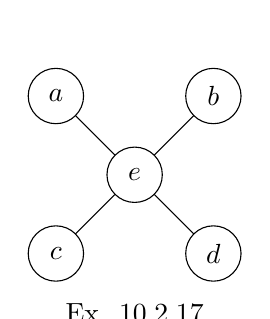
\begin{tikzpicture}[scale=1]
  \node[vtx] (a) at (-1,1) {$a$};
  \node[vtx] (b) at (1,1) {$b$};
  \node[vtx] (c) at (-1,-1) {$c$};
  \node[vtx] (d) at (1,-1) {$d$};
  \node[vtx] (e) at (0,0) {$e$};
  \draw (e)--(a) (e)--(b) (e)--(c) (e)--(d);
  \node at (0,-1.75) {Ex. 10.2.17};
\end{tikzpicture}
\hspace{2.0cm}
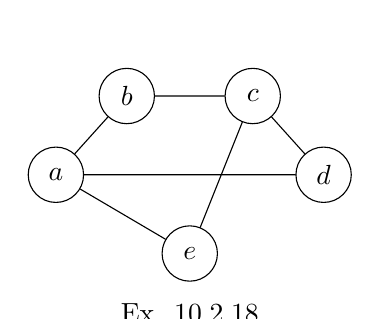
\begin{tikzpicture}[scale=1]
  \node[vtx] (a) at (-1.7,0) {$a$};
  \node[vtx] (b) at (-0.8,1) {$b$};
  \node[vtx] (c) at (0.8,1) {$c$};
  \node[vtx] (d) at (1.7,0) {$d$};
  \node[vtx] (e) at (0,-1) {$e$};
  \draw (a)--(b)--(c)--(d)--(a)--(e)--(c);
  \node at (0,-1.75) {Ex. 10.2.18};
\end{tikzpicture}
\end{center}

\subsection{Solution}

\subsubsection{Method 1: Explicit bipartitions}
\textbf{Definition used.} A graph $G=(V,E)$ is bipartite if $V$ can be written as a disjoint union
\[
V=V_1\sqcup V_2
\]
such that every edge has one endpoint in $V_1$ and the other endpoint in $V_2$.

\begin{enumerate}[label=(\alph*)]
  \item For Ex. 10.2.17, take
  \[
  V_1=\{a,b,c,d\},\qquad V_2=\{e\}.
  \]
  The edges are
  \[
  ea,\ eb,\ ec,\ ed,
  \]
  and each has one endpoint in $V_1$ and one endpoint in $V_2$. Hence the graph is bipartite.
  \[
  \boxed{\text{Ex. 10.2.17 is bipartite, with parts }\{a,b,c,d\}\text{ and }\{e\}.}
  \]

  \item For Ex. 10.2.18, take
  \[
  V_1=\{a,c\},\qquad V_2=\{b,d,e\}.
  \]
  The edges are
  \[
  ab,\ bc,\ cd,\ da,\ ae,\ ce.
  \]
  Checking them one by one,
  \[
  ab:V_1\text{--}V_2,
  \quad bc:V_2\text{--}V_1,
  \quad cd:V_1\text{--}V_2,
  \quad da:V_2\text{--}V_1,
  \quad ae:V_1\text{--}V_2,
  \quad ce:V_1\text{--}V_2.
  \]
  Hence every edge runs between the two parts.
  \[
  \boxed{\text{Ex. 10.2.18 is bipartite, with parts }\{a,c\}\text{ and }\{b,d,e\}.}
  \]
\end{enumerate}

\subsubsection{Method 2: Odd-cycle criterion}
\textbf{Theorem/criterion used.} A graph is bipartite if and only if it contains no cycle of odd length.

\begin{enumerate}[label=(\alph*)]
  \item Ex. 10.2.17 is a star $K_{1,4}$ with centre $e$. A tree has no cycles, hence has no odd cycles. Therefore it is bipartite.
  \[
  \boxed{\text{Ex. 10.2.17 is bipartite.}}
  \]

  \item In Ex. 10.2.18, the edge set is
  \[
  E=\{ab,bc,cd,da,ae,ce\}.
  \]
  There is no triangle: none of $ac,bd,be,de$ is an edge. Any cycle using $e$ must pass through both $a$ and $c$, and the two internally disjoint paths from $a$ to $c$ in the remaining graph are
  \[
  a-b-c\qquad\text{and}\qquad a-d-c,
  \]
  both of length $2$. Hence cycles through $e$ have length $4$, such as
  \[
  a-e-c-b-a
  \quad\text{or}\quad
  a-e-c-d-a.
  \]
  The cycle not using $e$ is
  \[
  a-b-c-d-a,
  \]
  also of length $4$. Thus all cycles are even. By the odd-cycle criterion, the graph is bipartite.
  \[
  \boxed{\text{Ex. 10.2.18 is bipartite.}}
  \]
\end{enumerate}

%====================================================
% QUESTION 3
%====================================================
\newpage
\section{Question 3 (Bipartiteness of complete graphs and cycles)}

\subsection{Problem}
For which values of $n$ are these graphs bipartite?
\begin{enumerate}[label=(\alph*)]
  \item $K_n$,
  \item $C_n$.
\end{enumerate}

\subsection{Solution}

\subsubsection{Method 1: Direct bipartition and odd-cycle analysis}
\begin{enumerate}[label=(\alph*)]
  \item For $K_n$, every pair of distinct vertices is adjacent.

  If $n=1$, then $K_1$ has no edge and is bipartite, for instance with parts $\{v\}$ and $\varnothing$.

  If $n=2$, then $K_2$ consists of a single edge and is bipartite with one endpoint in each part.

  If $n\ge 3$, choose three distinct vertices $u,v,w$. Since the graph is complete,
  \[
  uv,\ vw,\ wu\in E(K_n),
  \]
  so $u,v,w,u$ form a $3$-cycle. A bipartite graph has no odd cycle, so $K_n$ is not bipartite for $n\ge 3$.

  Hence
  \[
  \boxed{K_n\text{ is bipartite exactly for }n=1,2.}
  \]

  \item For $C_n$, the vertices can be written cyclically as
  \[
  v_1,v_2,\dots,v_n,v_1.
  \]
  If $n$ is even, put
  \[
  V_1=\{v_i:i\text{ is odd}\},\qquad V_2=\{v_i:i\text{ is even}\}.
  \]
  Each edge $v_iv_{i+1}$ joins an odd index to an even index, and the closing edge $v_nv_1$ also joins the two parts because $n$ is even. Hence $C_n$ is bipartite.

  If $n$ is odd, then $C_n$ itself is an odd cycle, so it is not bipartite.

  Therefore
  \[
  \boxed{C_n\text{ is bipartite exactly when }n\text{ is even}.}
  \]
\end{enumerate}

\subsubsection{Method 2: Chromatic-number criterion}
\textbf{Theorem/criterion used.} A graph is bipartite if and only if its chromatic number is at most $2$.

\begin{enumerate}[label=(\alph*)]
  \item The complete graph $K_n$ has chromatic number
  \[
  \chi(K_n)=n,
  \]
  because all $n$ vertices are pairwise adjacent and hence require $n$ distinct colours. Thus
  \[
  K_n\text{ is bipartite}
  \iff \chi(K_n)\le 2
  \iff n\le 2.
  \]
  For positive $n$, this gives
  \[
  \boxed{n=1\text{ or }n=2.}
  \]

  \item The cycle $C_n$ has chromatic number
  \[
  \chi(C_n)=
  \begin{cases}
  2, & n\text{ even},\\
  3, & n\text{ odd}.
  \end{cases}
  \]
  Therefore
  \[
  C_n\text{ is bipartite}
  \iff \chi(C_n)\le 2
  \iff n\text{ is even}.
  \]
  Hence
  \[
  \boxed{C_n\text{ is bipartite for all even }n.}
  \]
\end{enumerate}

%====================================================
% QUESTION 4
%====================================================
\newpage
\section{Question 4 (Degree sequences of complete bipartite graphs)}

\subsection{Problem}
The degree sequence of a graph is the sequence of the degrees of the vertices of the graph in nonincreasing order. For example, the degree sequence of the graph below is
\[
4,4,4,3,2,1,0.
\]

\begin{center}
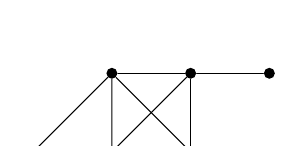
\begin{tikzpicture}[scale=1.0]
  \node[dotv] (x1) at (0,0) {};
  \node[dotv] (x2) at (1,1) {};
  \node[dotv] (x3) at (1,0) {};
  \node[dotv] (x4) at (2,1) {};
  \node[dotv] (x5) at (2,0) {};
  \node[dotv] (x6) at (3,1) {};
  \node[dotv] (x7) at (3,0) {};
  \draw (x1)--(x2)--(x3)--(x1);
  \draw (x2)--(x4)--(x5)--(x3);
  \draw (x2)--(x5);
  \draw (x3)--(x4);
  \draw (x4)--(x6);
\end{tikzpicture}
\end{center}

\noindent
What is the degree sequence of the bipartite graph $K_{2,3}$? How about $K_{m,n}$?

\subsection{Solution}

\subsubsection{Method 1: Direct use of the definition of $K_{m,n}$}
\textbf{Definition used.} The complete bipartite graph $K_{m,n}$ has a bipartition
\[
V=L\sqcup R,
\qquad |L|=m,
\qquad |R|=n,
\]
and every vertex in $L$ is adjacent to every vertex in $R$, with no edges inside $L$ or inside $R$.

For $K_{2,3}$, write
\[
|L|=2,
\qquad |R|=3.
\]
Each vertex in $L$ is adjacent to all $3$ vertices in $R$, so each has degree $3$. Each vertex in $R$ is adjacent to all $2$ vertices in $L$, so each has degree $2$. Therefore the degree sequence is
\[
\boxed{3,3,2,2,2.}
\]

For $K_{m,n}$:
\[
\deg(v)=n\quad (v\in L),
\qquad
\deg(w)=m\quad (w\in R).
\]
Thus, if $m\le n$, the nonincreasing degree sequence is
\[
\boxed{\underbrace{n,n,\dots,n}_{m\text{ terms}},\underbrace{m,m,\dots,m}_{n\text{ terms}}.}
\]
Equivalently, for arbitrary positive $m,n$, it is
\[
\boxed{
\underbrace{\max(m,n),\dots,\max(m,n)}_{\min(m,n)\text{ terms}},
\underbrace{\min(m,n),\dots,\min(m,n)}_{\max(m,n)\text{ terms}}.}
\]

\subsubsection{Method 2: Adjacency-row-sum computation}
Order the vertices so that the first $m$ vertices lie in $L$ and the last $n$ vertices lie in $R$. The adjacency matrix of $K_{m,n}$ has block form
\[
A=
\begin{pmatrix}
0_{m\times m} & J_{m\times n}\\
J_{n\times m} & 0_{n\times n}
\end{pmatrix},
\]
where $J$ is an all-ones matrix of the indicated size.

The degree of a vertex is the sum of the corresponding row of the adjacency matrix. Hence each of the first $m$ rows has sum $n$, and each of the last $n$ rows has sum $m$:
\[
\underbrace{n,\dots,n}_{m\text{ row sums}},
\underbrace{m,\dots,m}_{n\text{ row sums}}.
\]
Sorting in nonincreasing order gives the same answer as in Method 1. In particular,
\[
\boxed{K_{2,3}:\ 3,3,2,2,2,}
\]
and, if $m\le n$,
\[
\boxed{K_{m,n}:\ \underbrace{n,\dots,n}_{m\text{ terms}},\underbrace{m,\dots,m}_{n\text{ terms}}.}
\]

%====================================================
% QUESTION 5
%====================================================
\newpage
\section{Question 5 (Planarity after deleting one edge from $K_{3,3}$ and $K_5$)}

\subsection{Problem}
Prove that removing one edge from $K_{3,3}$ leads to a planar graph. How about $K_5$?

\subsection{Solution}

\subsubsection{Method 1: Explicit planar drawings}
It is enough to delete a representative edge, since all edges of $K_{3,3}$ are symmetric under graph isomorphism, and all edges of $K_5$ are symmetric under graph isomorphism.

\medskip
\noindent\textbf{Case 1: $K_{3,3}$ with one edge removed.}
Let the bipartition be
\[
\{1,2,3\}\sqcup\{4,5,6\}.
\]
Delete the edge $35$. Then the remaining graph has edge set
\[
\{14,15,16,24,25,26,34,36\}.
\]
A planar drawing is:

\begin{center}
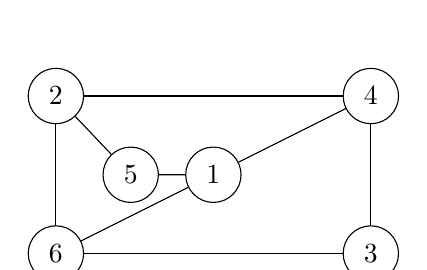
\begin{tikzpicture}[scale=1.0]
  \node[vtx] (two) at (-2,1) {$2$};
  \node[vtx] (four) at (2,1) {$4$};
  \node[vtx] (three) at (2,-1) {$3$};
  \node[vtx] (six) at (-2,-1) {$6$};
  \node[vtx] (one) at (0,0) {$1$};
  \node[vtx] (five) at (-1.05,0) {$5$};
  \draw (two)--(four)--(three)--(six)--(two);
  \draw (one)--(four) (one)--(six) (one)--(five);
  \draw (two)--(five);
\end{tikzpicture}
\end{center}

No two edges cross except at common endpoints. Hence $K_{3,3}-35$ is planar.

\medskip
\noindent\textbf{Case 2: $K_5$ with one edge removed.}
Delete the edge $35$. Then the remaining graph has all edges of $K_5$ except $35$:
\[
\{12,13,14,15,23,24,25,34,45\}.
\]
A planar drawing is:

\begin{center}
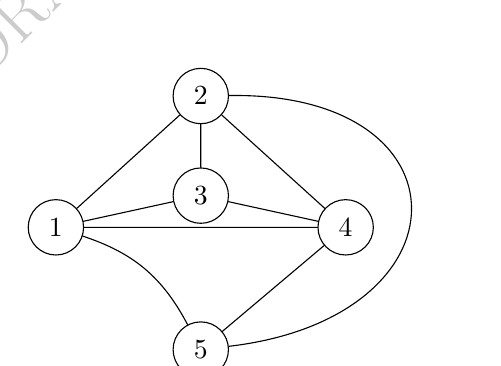
\begin{tikzpicture}[scale=1.15]
  \node[vtx] (1) at (-1.6,0) {$1$};
  \node[vtx] (2) at (0,1.45) {$2$};
  \node[vtx] (4) at (1.6,0) {$4$};
  \node[vtx] (3) at (0,0.35) {$3$};
  \node[vtx] (5) at (0,-1.35) {$5$};
  
  \draw (1)--(2)--(4)--(1);
  \draw (3)--(1) (3)--(2) (3)--(4);
  \draw (5) to[bend right=22] (1);
  \draw (5) to[bend left=0] (4);
  
  % Replaced the straight intersecting line with a control point curve
  \draw (5) .. controls (3,-1) and (3,1.5) .. (2);
\end{tikzpicture}
\end{center}
Again, no crossings occur. Therefore $K_5-35$ is planar.

Thus
\[
\boxed{\text{Removing one edge from either }K_{3,3}\text{ or }K_5\text{ gives a planar graph.}}
\]

\subsubsection{Method 2: Face-boundary planar embedding certificate}
\textbf{Criterion used.} A connected graph has a plane embedding if one can list face boundaries in which each edge appears exactly twice in total, once in each direction, and the cyclic incidences around vertices are consistent. Such a list is a combinatorial certificate for planarity.

\medskip
\noindent\textbf{Case 1: $K_{3,3}-35$.}
For the edge set
\[
E=\{14,15,16,24,25,26,34,36\},
\]
consider the following four face boundaries:
\[
1-4-2-5-1,
\qquad
1-5-2-6-1,
\qquad
1-4-3-6-1,
\qquad
2-4-3-6-2.
\]
Every listed boundary is a $4$-cycle. Checking edge appearances:
\[
\begin{array}{c|c}
\text{edge} & \text{faces containing it}\\ \hline
14 & (1\!-\!4\!-\!2\!-\!5\!-\!1),\ (1\!-\!4\!-\!3\!-\!6\!-\!1)\\
15 & (1\!-\!4\!-\!2\!-\!5\!-\!1),\ (1\!-\!5\!-\!2\!-\!6\!-\!1)\\
16 & (1\!-\!5\!-\!2\!-\!6\!-\!1),\ (1\!-\!4\!-\!3\!-\!6\!-\!1)\\
24 & (1\!-\!4\!-\!2\!-\!5\!-\!1),\ (2\!-\!4\!-\!3\!-\!6\!-\!2)\\
25 & (1\!-\!4\!-\!2\!-\!5\!-\!1),\ (1\!-\!5\!-\!2\!-\!6\!-\!1)\\
26 & (1\!-\!5\!-\!2\!-\!6\!-\!1),\ (2\!-\!4\!-\!3\!-\!6\!-\!2)\\
34 & (1\!-\!4\!-\!3\!-\!6\!-\!1),\ (2\!-\!4\!-\!3\!-\!6\!-\!2)\\
36 & (1\!-\!4\!-\!3\!-\!6\!-\!1),\ (2\!-\!4\!-\!3\!-\!6\!-\!2)
\end{array}
\]
Thus the graph admits a plane embedding with $4$ quadrilateral faces. Since
\[
|V|-|E|+|F|=6-8+4=2,
\]
this is consistent with Euler's formula.

\medskip
\noindent\textbf{Case 2: $K_5-35$.}
For the edge set
\[
E=\{12,13,14,15,23,24,25,34,45\},
\]
use the following six triangular face boundaries:
\[
1-2-3-1,
\quad
2-4-3-2,
\quad
4-1-3-4,
\quad
1-2-5-1,
\quad
2-4-5-2,
\quad
4-1-5-4.
\]
Each edge appears in exactly two face boundaries, and
\[
|V|-|E|+|F|=5-9+6=2.
\]
Hence this is a planar embedding certificate for $K_5-35$.

Therefore
\[
\boxed{K_{3,3}-e\text{ and }K_5-e\text{ are planar for every edge }e.}
\]

%====================================================
% QUESTION 6
%====================================================
\newpage
\section{Question 6 (Planar graphs with chromatic number $4$ and vertex deletion)}

\subsection{Problem}
\begin{enumerate}[label=(\alph*)]
  \item Find a planar graph $G$ such that $\chi(G)=4$.
  \item Prove that if, for a graph $G$, we remove one vertex and the edges incident to it, then the resulting graph $G'$ has chromatic number either $\chi(G)$ or $\chi(G)-1$.
\end{enumerate}

\subsection{Solution}

\subsubsection{Method 1: Direct example and colouring-extension proof}
\begin{enumerate}[label=(\alph*)]
  \item Take
  \[
  G=K_4.
  \]
  A planar drawing of $K_4$ is:
  \begin{center}
  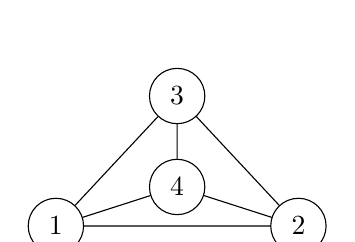
\begin{tikzpicture}[scale=1.1]
    \node[vtx] (1) at (-1.4,0) {$1$};
    \node[vtx] (2) at (1.4,0) {$2$};
    \node[vtx] (3) at (0,1.5) {$3$};
    \node[vtx] (4) at (0,0.45) {$4$};
    \draw (1)--(2)--(3)--(1);
    \draw (4)--(1) (4)--(2) (4)--(3);
  \end{tikzpicture}
  \end{center}
  It is planar because the drawing has no crossing edges.

  Since every pair of vertices in $K_4$ is adjacent, all four vertices must receive distinct colours in any proper colouring. Hence
  \[
  \chi(K_4)\ge 4.
  \]
  Four colours certainly suffice by assigning a different colour to each vertex, so
  \[
  \chi(K_4)=4.
  \]
  Therefore
  \[
  \boxed{G=K_4\text{ is planar and satisfies }\chi(G)=4.}
  \]

  \item Let $v\in V(G)$ be the removed vertex, and let
  \[
  G'=G-v.
  \]
  First, every proper colouring of $G$ restricts to a proper colouring of $G'$. Hence
  \[
  \chi(G')\le \chi(G).
  \]
  Second, take an optimal colouring of $G'$ using $\chi(G')$ colours. Colour the removed vertex $v$ with one new colour not used on $G'$. This gives a proper colouring of $G$ using at most $\chi(G')+1$ colours. Hence
  \[
  \chi(G)\le \chi(G')+1,
  \]
  which is equivalent to
  \[
  \chi(G)-1\le \chi(G').
  \]
  Combining the two inequalities gives
  \[
  \chi(G)-1\le \chi(G')\le \chi(G).
  \]
  Since chromatic numbers are integers,
  \[
  \boxed{\chi(G')\in\{\chi(G)-1,\chi(G)\}.}
  \]
\end{enumerate}

\subsubsection{Method 2 for Part (b): Minimality contradiction}
\textbf{Theorem/criterion used.} The chromatic number $\chi(H)$ is the least integer $k$ such that $H$ has a proper $k$-colouring.

Let $G'=G-v$.

The inequality
\[
\chi(G')\le \chi(G)
\]
follows because restricting a $\chi(G)$-colouring of $G$ to $G'$ remains proper.

It remains to prove that $\chi(G')$ cannot be less than $\chi(G)-1$. Suppose, for contradiction, that
\[
\chi(G')\le \chi(G)-2.
\]
Then $G'$ has a proper colouring using at most $\chi(G)-2$ colours. Colour $v$ with one additional new colour. This gives a proper colouring of $G$ using at most
\[
(\chi(G)-2)+1=\chi(G)-1
\]
colours, contradicting the minimality of $\chi(G)$.

Thus
\[
\chi(G')\ge \chi(G)-1.
\]
Together with $\chi(G')\le \chi(G)$, this gives
\[
\boxed{\chi(G')\in\{\chi(G)-1,\chi(G)\}.}
\]

%====================================================
% QUESTION 7
%====================================================
\newpage
\section{Question 7 (Five houses and two utilities)}

\subsection{Problem}
Can five houses be connected to two utilities without connections crossing?

\subsection{Solution}

\subsubsection{Method 1: Explicit planar drawing of $K_{2,5}$}
The situation is represented by the complete bipartite graph
\[
K_{2,5},
\]
where the two utilities form one part and the five houses form the other part.

A planar drawing is:

\begin{center}
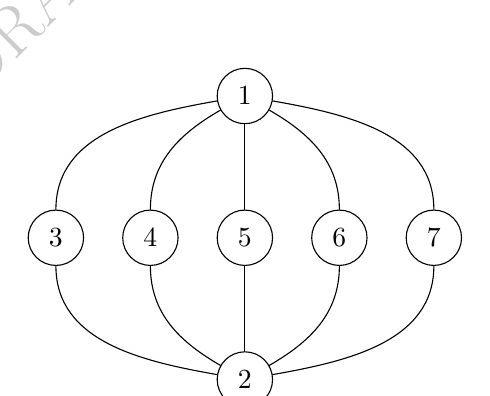
\begin{tikzpicture}[scale=1.0]
  \node[vtx] (u) at (0,1.8) {$1$};
  \node[vtx] (v) at (0,-1.8) {$2$};
  \node[vtx] (h1) at (-2.4,0) {$3$};
  \node[vtx] (h2) at (-1.2,0) {$4$};
  \node[vtx] (h3) at (0,0) {$5$};
  \node[vtx] (h4) at (1.2,0) {$6$};
  \node[vtx] (h5) at (2.4,0) {$7$};
  \draw (u) to[out=190,in=90] (h1);
  \draw (u) to[out=210,in=90] (h2);
  \draw (u)--(h3);
  \draw (u) to[out=-30,in=90] (h4);
  \draw (u) to[out=-10,in=90] (h5);
  \draw (v) to[out=170,in=-90] (h1);
  \draw (v) to[out=150,in=-90] (h2);
  \draw (v)--(h3);
  \draw (v) to[out=30,in=-90] (h4);
  \draw (v) to[out=10,in=-90] (h5);
\end{tikzpicture}
\end{center}

This drawing has no crossing edges. Therefore the five houses can be connected to the two utilities without crossings.
\[
\boxed{\text{Yes. The required graph is }K_{2,5}\text{, which is planar.}}
\]

\subsubsection{Method 2: General half-plane construction for $K_{2,n}$}
\textbf{Construction used.} For every positive integer $n$, the graph $K_{2,n}$ is planar: place the $n$ vertices of one part on a horizontal line, draw all edges from the first special vertex in the upper half-plane, and draw all edges from the second special vertex in the lower half-plane.

For $n=5$, place the five houses $h_1,\dots,h_5$ on a line, one utility $u$ above the line, and the other utility $v$ below the line. Draw the edges
\[
uh_i\quad (1\le i\le 5)
\]
as nonintersecting arcs in the upper half-plane, and draw the edges
\[
v h_i\quad (1\le i\le 5)
\]
as nonintersecting arcs in the lower half-plane. Upper-half-plane edges and lower-half-plane edges cannot cross except at the house vertices.

Hence this gives a planar embedding of $K_{2,5}$, so
\[
\boxed{\text{yes, five houses can be connected to two utilities without crossings.}}
\]

%====================================================
% QUESTION 8
%====================================================
\newpage
\section{Question 8 (Planarity of a six-vertex graph)}

\subsection{Problem}
Determine whether the given graph is planar. If so, draw it so that no edge cross.

\begin{center}
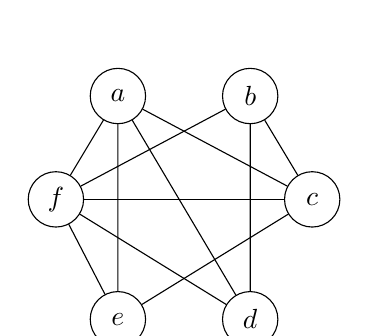
\begin{tikzpicture}[scale=1.05]
  \node[vtx] (a) at (-0.8,1.5) {$a$};
  \node[vtx] (b) at (0.8,1.5) {$b$};
  \node[vtx] (c) at (1.55,0.25) {$c$};
  \node[vtx] (d) at (0.8,-1.2) {$d$};
  \node[vtx] (e) at (-0.8,-1.2) {$e$};
  \node[vtx] (f) at (-1.55,0.25) {$f$};
  \draw (a)--(f)--(e)--(a);
  \draw (b)--(c)--(a);
  \draw (b)--(d)--(a);
  \draw (f)--(b);
  \draw (f)--(c);
  \draw (f)--(d);
  \draw (e)--(c);
\end{tikzpicture}
\end{center}

\subsection{Solution}

\subsubsection{Method 1: Explicit planar redrawing}
The graph has edge set
\[
E=\{af,ae,ad,ac,bf,bc,bd,cf,df,ef,ce\}.
\]
A planar representation is:

\begin{center}
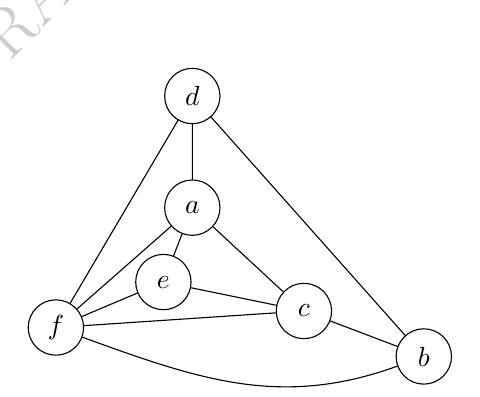
\begin{tikzpicture}[scale=1.05]
  \node[vtx] (d) at (0,2.8) {$d$};
  \node[vtx] (a) at (0,1.45) {$a$};
  \node[vtx] (f) at (-1.65,0) {$f$};
  \node[vtx] (e) at (-0.35,0.55) {$e$};
  \node[vtx] (c) at (1.35,0.2) {$c$};
  \node[vtx] (b) at (2.8,-0.35) {$b$};

  \draw (d)--(a)--(f)--(d);
  \draw (a)--(e)--(f);
  \draw (a)--(c)--(e);
  \draw (f)--(c);
  \draw (c)--(b)--(d);
  \draw (f) to[out=-20,in=200] (b);
\end{tikzpicture}
\end{center}

The displayed drawing contains all edges
\[
 af,ae,ad,ac,bf,bc,bd,cf,df,ef,ce
\]
and has no crossing edges. Therefore the graph is planar.
\[
\boxed{\text{The given graph is planar.}}
\]

\subsubsection{Method 2: Face-boundary certificate}
\textbf{Criterion used.} A plane drawing can be certified by listing face boundaries so that each edge is incident with exactly two faces and Euler's formula is satisfied.

For the edge set
\[
E=\{af,ae,ad,ac,bf,bc,bd,cf,df,ef,ce\},
\]
consider the following face boundaries:
\[
\begin{aligned}
&d-a-f-d,\\
&a-d-b-c-a,\\
&a-f-e-a,\\
&a-e-c-a,\\
&f-e-c-f,\\
&f-c-b-f,\\
&f-d-b-f.
\end{aligned}
\]
Every edge appears in exactly two of these face boundaries:
\[
\begin{array}{c|c}
\text{edge} & \text{two incident faces}\\ \hline
ad & d-a-f-d,\ a-d-b-c-a\\
af & d-a-f-d,\ a-f-e-a\\
df & d-a-f-d,\ f-d-b-f\\
bd & a-d-b-c-a,\ f-d-b-f\\
bc & a-d-b-c-a,\ f-c-b-f\\
ac & a-d-b-c-a,\ a-e-c-a\\
ae & a-f-e-a,\ a-e-c-a\\
ef & a-f-e-a,\ f-e-c-f\\
ce & a-e-c-a,\ f-e-c-f\\
cf & f-e-c-f,\ f-c-b-f\\
bf & f-c-b-f,\ f-d-b-f
\end{array}
\]
Also,
\[
|V|-|E|+|F|=6-11+7=2.
\]
Thus these face boundaries give a planar embedding certificate. Therefore
\[
\boxed{\text{the graph is planar.}}
\]

%====================================================
% QUESTION 9
%====================================================
\newpage
\section{Question 9 (Chromatic number after deleting any vertex)}

\subsection{Problem}
\begin{enumerate}[label=(\alph*)]
  \item Is there a planar simple connected graph with more than $3$ vertices, such that removing any vertex and incident edges from it results in $\chi(G)-1$? If so, find one.
  \item Is there a planar simple connected graph with $5$ or less vertices, such that removing any vertex and incident edges from it results in $\chi(G)$? If so, find one.
\end{enumerate}

\subsection{Solution}

\subsubsection{Method 1: Direct examples and verification}
\begin{enumerate}[label=(\alph*)]
  \item Take
  \[
  G=K_4.
  \]
  The graph $K_4$ is planar, simple, connected, and has $4>3$ vertices. Since every two vertices of $K_4$ are adjacent,
  \[
  \chi(K_4)=4.
  \]
  Removing any vertex from $K_4$ leaves $K_3$, and
  \[
  \chi(K_3)=3=4-1=\chi(K_4)-1.
  \]
  Hence
  \[
  \boxed{G=K_4\text{ works for part (a).}}
  \]

  \item Take
  \[
  G=C_4.
  \]
  The graph $C_4$ is planar, simple, connected, and has $4\le 5$ vertices. Since $C_4$ is an even cycle,
  \[
  \chi(C_4)=2.
  \]
  Removing any vertex from $C_4$ leaves a path on $3$ vertices, namely $P_3$. Since $P_3$ has at least one edge, it is not $1$-colourable; since it is a path, it is $2$-colourable. Therefore
  \[
  \chi(P_3)=2=\chi(C_4).
  \]
  Hence
  \[
  \boxed{G=C_4\text{ works for part (b).}}
  \]
\end{enumerate}

\subsubsection{Method 2: Vertex-transitivity and chromatic invariants}
\textbf{Principle used.} If a graph is vertex-transitive, then deleting any vertex produces isomorphic induced subgraphs. Hence it is enough to check one deleted vertex.

\begin{enumerate}[label=(\alph*)]
  \item The graph $K_4$ is vertex-transitive. Since
  \[
  K_4-v\cong K_3
  \]
  for every $v\in V(K_4)$, and since
  \[
  \chi(K_4)=4,
  \qquad
  \chi(K_3)=3,
  \]
  deleting any vertex reduces the chromatic number by exactly one:
  \[
  \chi(K_4-v)=\chi(K_4)-1.
  \]
  The graph is planar, simple, connected, and has more than $3$ vertices. Thus
  \[
  \boxed{K_4\text{ is a valid example.}}
  \]

  \item The graph $C_4$ is vertex-transitive. For every $v\in V(C_4)$,
  \[
  C_4-v\cong P_3.
  \]
  Since $C_4$ is an even cycle,
  \[
  \chi(C_4)=2.
  \]
  Since $P_3$ is a nontrivial path,
  \[
  \chi(P_3)=2.
  \]
  Therefore
  \[
  \chi(C_4-v)=\chi(C_4)
  \]
  for every vertex $v$. The graph is planar, simple, connected, and has at most $5$ vertices. Hence
  \[
  \boxed{C_4\text{ is a valid example.}}
  \]
\end{enumerate}

\end{document}